%% ============================================================
%% GHG Quantification --Thailand Rice CH4 Emissions
%% IPEN6100F Final Project | Template: olplainarticle
%% Compile: pdflatex ->bibtex ->pdflatex ->pdflatex
%% ============================================================

\documentclass[fleqn,10pt]{olplainarticle}

\usepackage{newtxtext,newtxmath}   % Times New Roman text + math
\usepackage{setspace}              % line spacing
\usepackage{microtype}
\usepackage{booktabs}
\usepackage{multirow}
\usepackage{float}
\usepackage{placeins}
\usepackage{amsmath}
\usepackage{array}
\newcolumntype{L}[1]{>{\raggedright\arraybackslash}p{#1}}

\title{Price Policy as a Driver of Agricultural Methane: Evidence from
       Thailand's Rice Sector, 1961--2024}

\author[1]{Sirawit Tangchiitwatthanakon}
\affil[1]{The Hong Kong University of Science and Technology (Guangzhou), Guangzhou, China}

\keywords{methane emissions; paddy rice cultivation; greenhouse gas inventory;
          IPCC Tier~1 methodology; Thailand; subnational spatial analysis;
          agricultural price support; Nationally Determined Contribution;
          alternate wetting and drying}

\begin{abstract}
Rice paddies are a major source of methane (CH\textsubscript{4}), a greenhouse gas with a
100-year global warming potential (GWP\textsubscript{100}) of 28.
Thailand, one of the world's top rice exporters, cultivates approximately 11~million
hectares annually, making accurate CH\textsubscript{4} estimation essential for national
climate reporting.
This study applies IPCC 2006 Tier~1 at two scales (a national time series 1961--2024
and a 77-province analysis 2022--2024) to quantify rice CH\textsubscript{4} emissions
and examine how the \textit{structural design} of price-support programmes determines
their emission impact.
National emissions averaged \textbf{1,420~Gg~CH\textsubscript{4}~yr\textsuperscript{-1}}
(39.8~Mt~CO\textsubscript{2}e), peaking at 1,884~Gg in 2012 before falling to 1,726~Gg
in 2024; the Northeast accounts for 55\% of provincial emissions.
The 2011--2014 Rice Pledging Scheme, an unlimited price guarantee at 40--50\% above
market, added an estimated 988,000~ha beyond the price effect alone ($p < 0.001$).
A counterfactual estimate shows that a per-household area cap applied from 2011 would
have avoided approximately \textbf{606~Gg~CH\textsubscript{4}} (17.0~Mt~CO\textsubscript{2}e)
over four years, more than five times the annual mitigation potential of full
Alternate Wetting and Drying (AWD) adoption across all irrigated provinces.
Emission intensity fell 44\% (92.5 to 51.4~kg~CH\textsubscript{4}~t\textsuperscript{-1})
as yields improved, yet absolute emissions rose 84\%: a rebound effect in which
yield gains raised the profitability of rice cultivation and attracted area expansion.
These findings indicate that Thailand's NDC agriculture targets are more sensitive
to the \textit{design} of price-support programmes than to yield improvement or
field-level mitigation technologies alone.
\end{abstract}

\begin{document}
\onehalfspacing

\flushbottom
\maketitle
\thispagestyle{empty}

% =============================================================
\section*{Introduction}
% =============================================================

Thailand is one of the world's great rice economies.
Consistently among the top three rice exporters globally \citep{faostat2026},
the country devotes over 11~million hectares to paddy cultivation each year, a landscape
that shapes livelihoods, food security, and foreign exchange across Southeast
Asia.
These same flooded fields also produce a potent greenhouse gas.
Kept underwater for months, paddy fields support microbes that generate
methane (CH\textsubscript{4}), a gas with a GWP\textsubscript{100} of 28
that has contributed approximately 20\% of human-caused radiative forcing
since pre-industrial times \citep{myhre2013}.
Agriculture as a whole contributes 10--12\% of global greenhouse gas (GHG)
emissions, and flooded rice paddies alone account for 25--60~Tg~CH\textsubscript{4}~yr\textsuperscript{-1},
roughly 10--12\% of the global CH\textsubscript{4} budget
\citep{neue1993, yan2009, smith2014}.

In flooded fields, microbes break down organic matter without oxygen and release
CH\textsubscript{4}; the gas escapes to the atmosphere mainly through hollow
channels in the rice plant's stem \citep{neue1993}.
Because emission rates scale directly with flooded area and growing period
\citep{ipcc2006}, any expansion of rice cultivation (more land planted, more
seasons per year) directly increases emissions.
This study finds that Thailand's paddies emitted on average
1,420~Gg~CH\textsubscript{4}~yr\textsuperscript{-1} over 1961--2024,
and that over the period for which price data are available (2007--2024),
farm-gate price policy drives year-to-year area swings, with the 2011--2014 price-support scheme coinciding
with the 64-year emission peak.

Despite this striking episode, the quantitative link between rice price
support and CH\textsubscript{4} emissions has received limited scientific
attention.
While broader modelling studies have examined how agricultural subsidies
and trade policy reshape land use and GHG emissions across multiple commodities
\citep{mosnier2014, frank2018}, few have applied this framework specifically
to price-support mechanisms in tropical rice systems.
Furthermore, the spatial distribution of Thailand's rice emissions at
provincial scale remains poorly documented.

This study pursues three objectives:
\begin{enumerate}[noitemsep]
  \item to quantify the long-term (1961--2024) national CH\textsubscript{4} trend
        and its statistical characteristics using FAOSTAT data;
  \item to map province-scale rice CH\textsubscript{4} emissions and emission
        intensity across Thailand for 2022--2024 using OAE sub-national data; and
  \item to examine the relationship between farm-gate rice price, harvested area,
        and CH\textsubscript{4} emissions, and discuss implications for Thai rice policy.
\end{enumerate}

% =============================================================
\section*{Data and Methodology}
% =============================================================

\subsection*{Study area}

Thailand (5$^\circ$37'--20$^\circ$27'N, 97$^\circ$22'--105$^\circ$38'E) covers 513,120~km\textsuperscript{2}
and comprises 77 provinces in four macro-regions: North, Northeast, Central, and South.
The Northeast Plateau (Khorat Plateau) is the largest rice-producing region,
dominated by rainfed single-crop paddy.
The Central Plains (Chao Phraya basin) supports double-cropped irrigated paddy
with high yields.
Northern valleys contain irrigated main-season paddy, while the South cultivates
small rice areas amid rubber and oil palm.

\subsection*{Data sources}

\textbf{National activity data (1961--2024).}
Annual rice harvested area was obtained from FAOSTAT \citep{faostat2026}
(element code~5312), spanning 64 years.
FAOSTAT harvested area counts each crop season separately, making it compatible
with a per-season emission factor.

\textbf{Provincial activity data (2022--2024).}
Sub-national harvested area and production by province were obtained from the
Office of Agricultural Economics (OAE) \citep{oae2024} for the main season
(\textit{khao na pi}) and dry/irrigated season
(\textit{khao na prang}) across all 77 provinces.
Data were released as PDF tables; a custom \texttt{pdfplumber}-based Python
parser was developed to extract and clean records, handling PDF number-splitting
artefacts and Thai character encoding.
Areas were converted from rai to hectares (1~ha = 6.25~rai).

\textbf{Rice farm-gate prices (2007--2024).}
Monthly farm-gate paddy prices (THB per tonne, 15\% moisture content) were
obtained from OAE \citep{oae2024} and converted to annual averages.
This price series was merged with FAOSTAT national data for policy analysis.

\textbf{Spatial boundaries.}
Province boundaries from GADM~4.1 Level~1 \citep{gadm2024} were used for
choropleth mapping.

\subsection*{IPCC 2006 Tier 1 emission calculation}

CH\textsubscript{4} emissions follow IPCC 2006 Guidelines, Vol.~4, Ch.~5
\citep{ipcc2006}, Equation~5.1:

\begin{equation}
  \text{CH}_{4,i} = \text{EF}_i \times A_i \times 10^{-6}
  \label{eq:ch4}
\end{equation}

\noindent where $\text{CH}_{4,i}$ is annual emission (Gg~yr\textsuperscript{-1}),
$A_i$ is harvested area (ha), and the seasonal emission factor is:

\begin{equation}
  \text{EF}_i = \text{EF}_c \times \text{SF}_{w} \times \text{SF}_{p}
               \times \text{SF}_{o} \times t_{p}
  \label{eq:ef}
\end{equation}

This study applies Tier~1 default scaling factors: $\text{SF}_w = \text{SF}_p
= \text{SF}_o = 1.0$ (continuously flooded baseline, no pre-season flooding
$>$30 days, no organic amendments), consistent with IPCC Tables~5.12--5.14
\citep{ipcc2006}.
This yields emission factors of 153.4~kg~ha\textsuperscript{-1} for the main season
and 144.3~kg~ha\textsuperscript{-1} for the dry/irrigated season (Table~\ref{tab:ef}).
CO\textsubscript{2}-equivalent emissions use GWP\textsubscript{100} = 28
\citep{myhre2013}.

\begin{table}[!htbp]
\centering
\caption{IPCC 2006 Tier~1 parameters used in this study.
         $\text{EF}_c$ from Table~5.11; scaling factors from Tables~5.12--5.14
         \citep{ipcc2006}; GWP from \cite{myhre2013}.}
\label{tab:ef}
\begin{tabular}{@{}lll@{}}
\toprule
\textbf{Parameter} & \textbf{Value} & \textbf{Source} \\
\midrule
$\text{EF}_c$ & 1.30~kg~CH\textsubscript{4}~ha\textsuperscript{-1}~day\textsuperscript{-1} & IPCC Table~5.11 \\
$\text{SF}_w$ & 1.00 (continuously flooded baseline) & IPCC Table~5.12 \\
$\text{SF}_p$ & 1.00 ($\leq$180 days pre-season non-flooded) & IPCC Table~5.13 \\
$\text{SF}_o$ & 1.00 (no organic amendments) & IPCC Table~5.14 \\
\midrule
$t_p$ (main season)  & 118 days & \cite{buddhaboon2011} \\
$t_p$ (dry season)   & 111 days & \cite{buddhaboon2011} \\
\textbf{EF (main)} & \textbf{153.4 kg~ha\textsuperscript{-1}~season\textsuperscript{-1}} & Derived \\
\textbf{EF (dry)}  & \textbf{144.3 kg~ha\textsuperscript{-1}~season\textsuperscript{-1}} & Derived \\
GWP\textsubscript{100} (CH\textsubscript{4}) & 28 & AR5, \cite{myhre2013}$^{\dagger}$ \\
\bottomrule
\end{tabular}
\end{table}

\subsection*{Emission intensity and statistical analysis}

Emission intensity was calculated as:
\begin{equation}
  I_i = \frac{\text{CH}_{4,i} \times 10^6}{P_i}
  \label{eq:intensity}
\end{equation}
\noindent where $I_i$ is emission intensity (kg~CH\textsubscript{4}~t\textsuperscript{-1}~rice)
and $P_i$ is rice production (tonnes).
Linear regression on annual CH\textsubscript{4} values captures the long-term trend.
Emission intensity (kg~CH\textsubscript{4}~t\textsuperscript{-1} rice) was calculated
for 1961--2024 to assess whether higher yields have reduced the climate cost per
tonne of rice.
Pearson correlation and simple linear regression were used to test the
relationship between farm-gate price and harvested area, with statistical
significance assessed at $\alpha = 0.05$.
As a robustness check, a multivariate OLS model including a binary
policy dummy variable ($D_t = 1$ for 2011--2014 Pledging Scheme years,
0 otherwise) was estimated:
\begin{equation}
  A_t = \beta_0 + \beta_1 P_t + \beta_2 D_t + \varepsilon_t
  \label{eq:dummy}
\end{equation}
where $A_t$ is national harvested area and $P_t$ is annual farm-gate price.
Residual autocorrelation was assessed via the Durbin--Watson statistic
\citep{durbinwatson1950}; Newey--West heteroskedasticity- and
autocorrelation-consistent standard errors \citep{neweywest1987} are
reported for all OLS models as a background correction to account for
potential serial dependence in annual time-series data.

% =============================================================
\section*{Results and Discussion}
% =============================================================

\subsection*{National emission trends and yield paradox (1961--2024)}

Figure~\ref{fig:national} presents the 64-year time series of harvested area
and CH\textsubscript{4} emissions with a fitted linear trend.

\begin{figure}[!htbp]
\centering
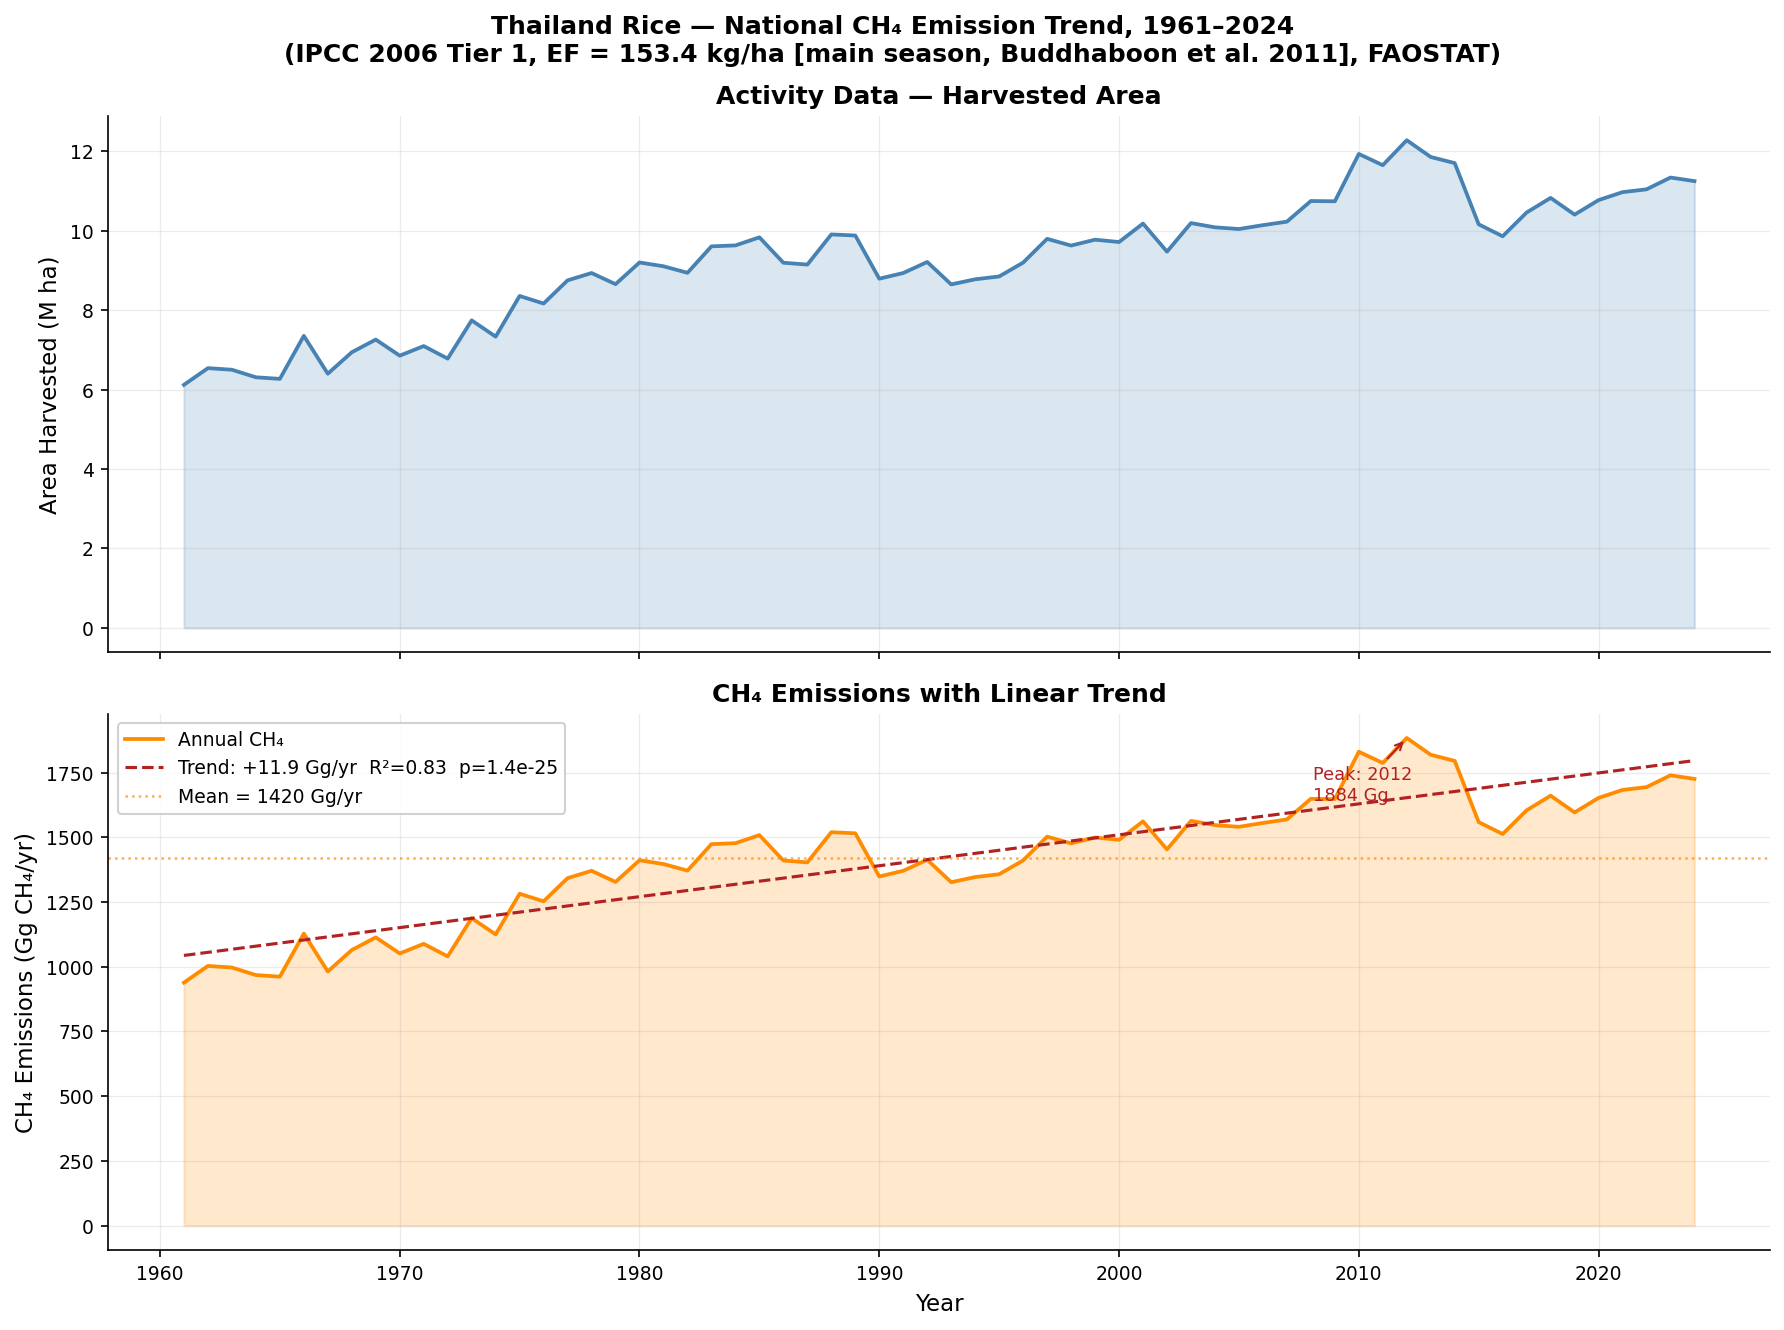
\includegraphics[width=0.96\linewidth]{plot1_national_trend.png}
\caption{National trends in Thailand rice cultivation, 1961--2024.
         \textbf{Top}: Total harvested area (M~ha).
         \textbf{Bottom}: CH\textsubscript{4} emissions
         (Gg~CH\textsubscript{4}~yr\textsuperscript{-1}) with linear trend
         (dashed red) and long-term mean (dotted).
         Source: \cite{faostat2026}; IPCC 2006 Tier~1; authors' calculation.}
\label{fig:national}
\end{figure}

Over the full study period, Thailand's mean annual rice CH\textsubscript{4}
emission was \textbf{1,420~Gg~CH\textsubscript{4}~yr\textsuperscript{-1}}
(39.8~Mt~CO\textsubscript{2}e; Table~\ref{tab:national}).
Linear regression reveals a statistically significant upward trend of
\textbf{+12.0~Gg~CH\textsubscript{4}~yr\textsuperscript{-1}}
($R^2 = 0.830$, $p = 1.4 \times 10^{-25}$), confirming that emissions
have risen substantially over six decades.
Emissions grew from 939~Gg in 1961 to a peak of \textbf{1,884~Gg in 2012}
(an increase of 101\%), before declining to 1,726~Gg by 2024.
The 2024 value (48.3~Mt~CO\textsubscript{2}e) represents approximately 13\%
of Thailand's total national GHG emissions, based on the \textasciitilde{}375~Mt~CO\textsubscript{2}e
total reported in Thailand's Third Biennial Update Report \citep{tgo2022}.

The long-run growth reflects two overlapping forces.
From the 1960s through the 1980s, government investment in irrigation
infrastructure and the adoption of high-yielding varieties under Thailand's
Green Revolution allowed farmers to cultivate more land and add a second crop
per year in irrigated areas.
From the 1990s onward, rising global export demand created a sustained
incentive to expand production, as Thailand competed with Vietnam and other
regional exporters for world market share.
Together, these forces drove a steady climb in harvested area and, because
CH\textsubscript{4} scales directly with flooded area under Tier~1, in
emissions.
The 2012 peak stands apart: it was not driven by these long-run structural
forces but by a government scheme that made unlimited area expansion
immediately profitable (discussed below).

\begin{table}[!htbp]
\centering
\caption{Summary statistics of national rice CH\textsubscript{4} emissions,
         Thailand, 1961--2024.}
\label{tab:national}
\begin{tabular}{@{}lrl@{}}
\toprule
\textbf{Indicator} & \textbf{Value} & \textbf{Unit} \\
\midrule
Mean harvested area (1961--2024)         & 9.26    & M~ha~yr\textsuperscript{-1} \\
Mean CH\textsubscript{4} (1961--2024)    & 1,420.0 & Gg~CH\textsubscript{4}~yr\textsuperscript{-1} \\
Minimum CH\textsubscript{4} (1961)       & 938.8   & Gg~CH\textsubscript{4}~yr\textsuperscript{-1} \\
Peak CH\textsubscript{4} (2012)          & 1,883.6 & Gg~CH\textsubscript{4}~yr\textsuperscript{-1} \\
CH\textsubscript{4} in 2024              & 1,725.5 & Gg~CH\textsubscript{4}~yr\textsuperscript{-1} \\
Linear trend                             & +12.0   & Gg~CH\textsubscript{4}~yr\textsuperscript{-1} \\
$R^2$ / $p$-value                        & 0.830 / $<$0.001 & --- \\
Change 1961--2024                        & +83.8   & \% \\
\bottomrule
\end{tabular}
\end{table}

Despite rising absolute emissions, Thailand's emission intensity (CH\textsubscript{4}
per tonne of rice produced) has declined sharply over six decades
(Figure~\ref{fig:efficiency}).
Intensity fell from \textbf{92.5~kg~CH\textsubscript{4}~t\textsuperscript{-1}}
in 1961 to \textbf{51.4~kg~CH\textsubscript{4}~t\textsuperscript{-1}} in 2024,
a reduction of 44\%, with a highly significant downward trend of
$-0.730$~kg~t\textsuperscript{-1}~yr\textsuperscript{-1}
($R^2 = 0.892$, $p < 0.001$).

\begin{figure}[!htbp]
\centering
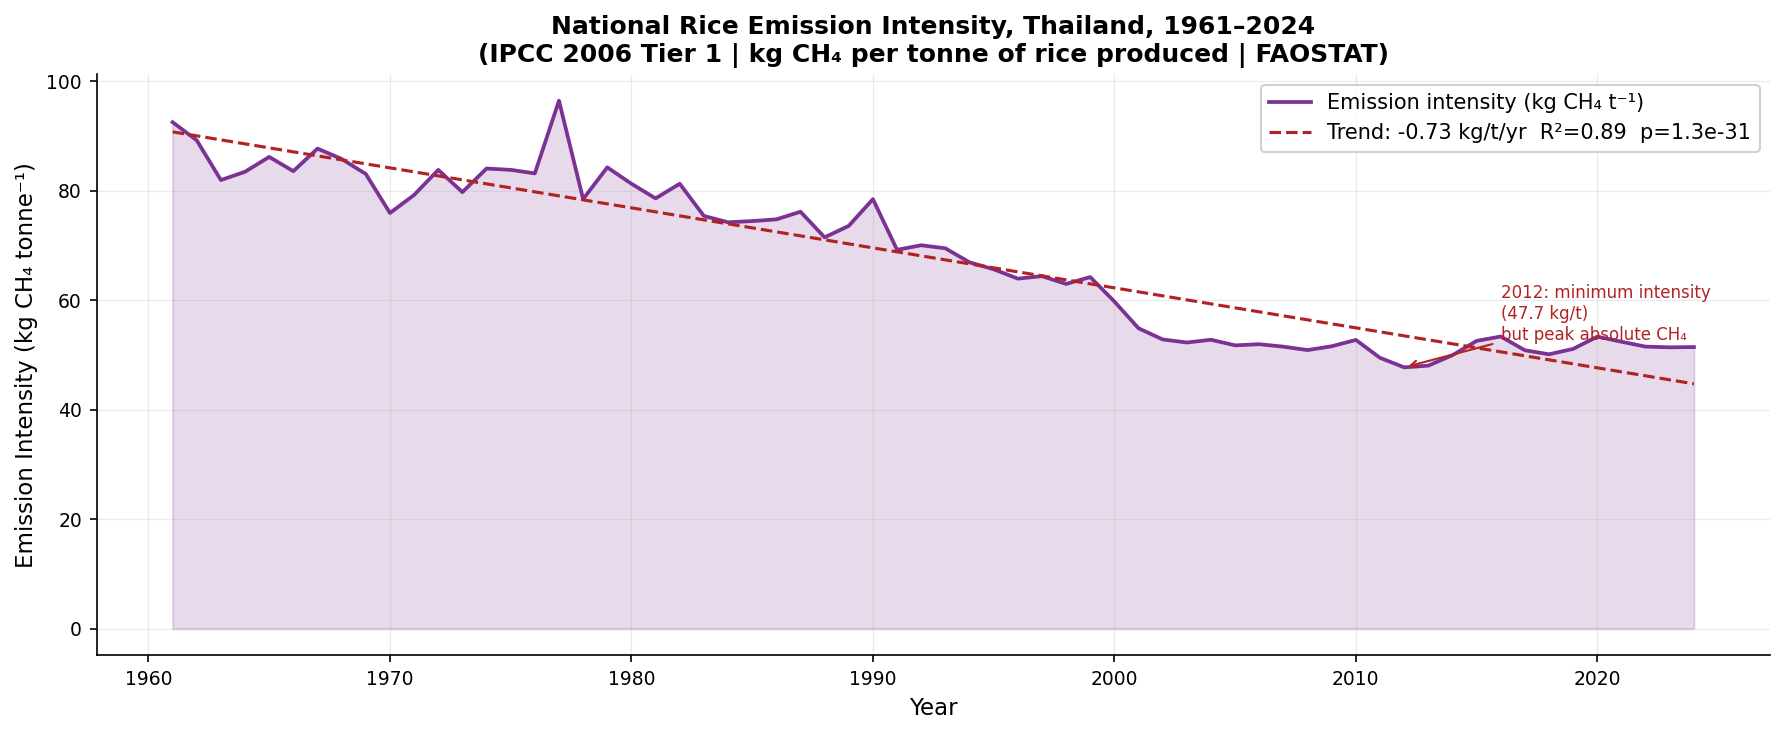
\includegraphics[width=0.96\linewidth]{plot8_yield_efficiency.png}
\caption{National rice emission intensity (kg~CH\textsubscript{4} per tonne
         of rice produced), Thailand, 1961--2024, with linear trend (dashed red).
         Intensity has declined 44\% over six decades as yield growth outpaced
         area expansion.
         Source: \cite{faostat2026}; IPCC 2006 Tier~1; authors' calculation.}
\label{fig:efficiency}
\end{figure}

This is a real \textbf{food-system efficiency gain}: Thailand now produces
each tonne of rice at 44\% lower climate cost than in 1961.
The improvement reflects nationwide adoption of improved seed varieties
and expanded irrigation, which raised average yields across all regions.
Irrigated areas, particularly the Central Plains double-crop system,
contributed disproportionately high yields, pulling the national average up
and reducing the CH\textsubscript{4} cost per tonne of rice produced.
It does \textbf{not} mean less methane per hectare.
Under Tier~1, intensity is simply $\text{EF}_c \times t_p$ divided by yield, so the
decline is automatic when yields rise, not a sign of improved field-level water
management.
Whether actual CH\textsubscript{4} flux per hectare has changed requires Tier~2 field
measurements to detect.
Finally, total emissions still rose 84\% over the same period, because farmers planted
more land faster than yields improved.
The minimum intensity year was \textbf{2012} (47.7~kg~t\textsuperscript{-1}):
the Pledging Scheme's output incentive drove yields to record levels in
Central irrigated areas, inadvertently producing Thailand's most food-efficient
harvest on a per-tonne basis, the same year absolute emissions peaked.

This juxtaposition reveals a critical paradox for climate policy: \textbf{yield
improvement and absolute emission reduction do not automatically co-occur}.
Under Tier~1, higher yield reduces emission intensity mechanically (the same
CH\textsubscript{4} is spread over more tonnes of rice), but leaves absolute
emissions entirely unchanged: only area matters.
Beyond the accounting identity, yield gains can actively \textit{increase}
absolute emissions through a rebound effect: more profitable production per
hectare raises the return to planting, attracting more farmers and pushing
marginal land into cultivation.
Thailand's 64-year record illustrates this precisely: the Green Revolution
raised both yields \textit{and} planted area simultaneously, so absolute
emissions climbed even as intensity fell.
The implication for policy is direct: programmes that raise on-farm yields
without constraining area (through caps, zoning, or purchase limits) may
inadvertently drive emission increases.
Yield improvement reduces absolute CH\textsubscript{4} only if it enables
the \textit{same total production on less land}, a land-sparing outcome that
requires deliberate area management, not just better agronomy.

\FloatBarrier
\subsection*{Spatial distribution of the climate cost}

Figure~\ref{fig:choropleth} maps mean annual CH\textsubscript{4} emissions
per province for 2022--2024.
The Northeast clearly dominates the spatial pattern, consistent with its
large paddy area on the Khorat Plateau.

\begin{figure}[!htbp]
\centering
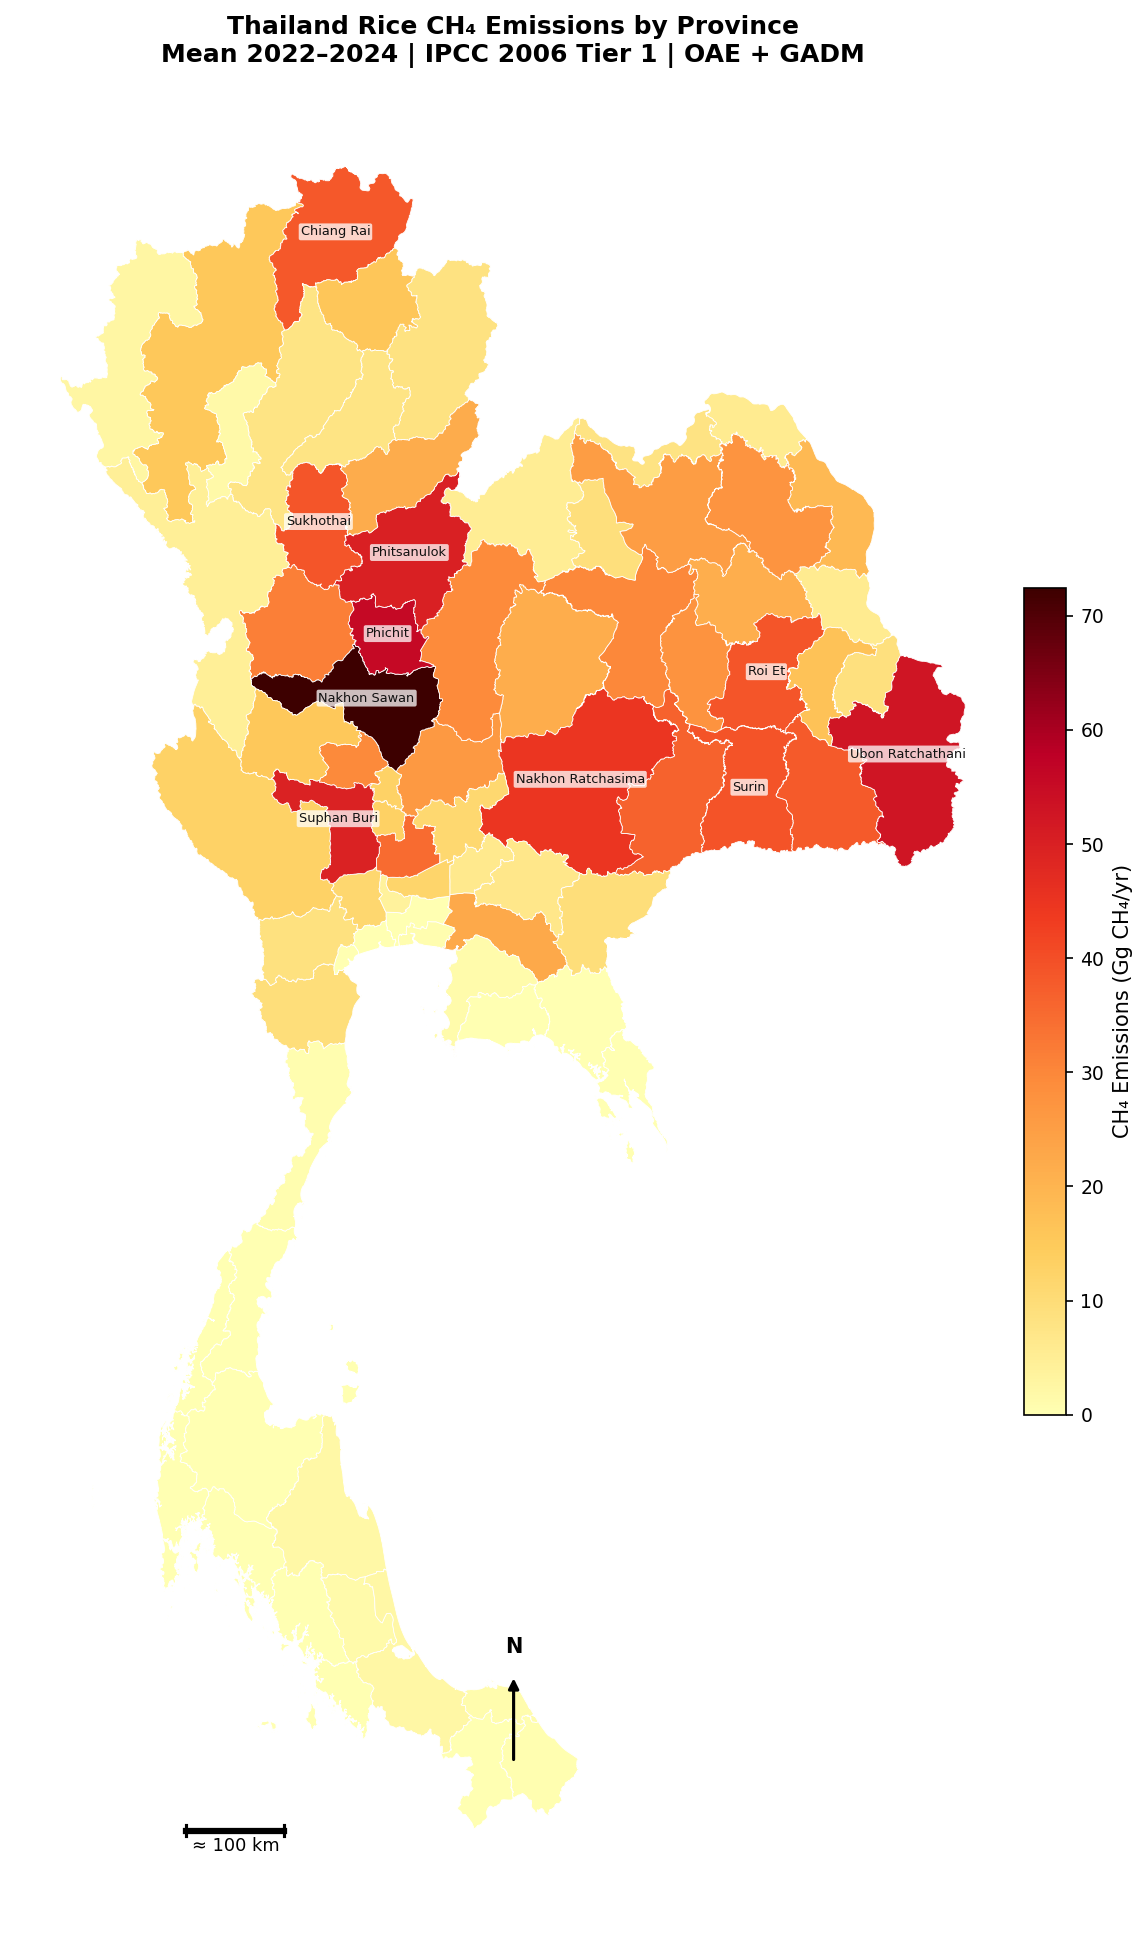
\includegraphics[width=0.72\linewidth]{plot4_choropleth.png}
\caption{Choropleth map of mean annual rice CH\textsubscript{4} emissions
         by province, Thailand, 2022--2024.
         Continuous colour scale (pale yellow = low, near-black = high).
         Top-10 emitting provinces labelled.
         Source: \cite{oae2024}; \cite{gadm2024}; authors' calculation.}
\label{fig:choropleth}
\end{figure}

\begin{table}[!htbp]
\centering
\caption{Top 10 rice-CH\textsubscript{4}-emitting provinces, Thailand,
         mean annual 2022--2024 (IPCC 2006 Tier~1).}
\label{tab:top10}
\begin{tabular}{@{}clcrrr@{}}
\toprule
\textbf{Rk} & \textbf{Province} & \textbf{Region} &
  \textbf{Area (kha)} &
  \textbf{CH\textsubscript{4} (Gg~yr\textsuperscript{-1})} &
  \textbf{Intensity (kg~t\textsuperscript{-1})} \\
\midrule
1  & Ubon Ratchathani   & Northeast & 662 & 101.4 & 66.8 \\
2  & Nakhon Ratchasima  & Northeast & 564 &  86.3 & 63.1 \\
3  & Surin              & Northeast & 491 &  75.2 & 63.9 \\
4  & Roi Et             & Northeast & 490 &  74.8 & 66.8 \\
5  & Si Sa Ket          & Northeast & 477 &  73.0 & 67.1 \\
6  & Nakhon Sawan       & Central   & 478 &  72.4 & 40.5 \\
7  & Buri Ram           & Northeast & 459 &  70.3 & 66.0 \\
8  & Khon Kaen          & Northeast & 376 &  57.5 & 69.0 \\
9  & Phichit            & North     & 368 &  55.7 & 39.4 \\
10 & Maha Sarakham      & Northeast & 347 &  53.0 & 63.8 \\
\bottomrule
\multicolumn{6}{@{}l@{}}{\footnotesize kha = thousand ha; intensity = kg CH\textsubscript{4} per tonne rice produced.}
\end{tabular}
\end{table}

Table~\ref{tab:top10} lists the ten highest-emitting provinces.
\textbf{Ubon Ratchathani} (Northeast) leads with 101.4~Gg~yr\textsuperscript{-1},
followed by \textbf{Nakhon Ratchasima} (Northeast, 86.3~Gg) and
\textbf{Surin} (Northeast, 75.2~Gg).
The first Central province to appear is \textbf{Nakhon Sawan} at rank~6
(72.4~Gg), which benefits from both large irrigated area and a productive
double-cropping system.
The full provincial ranking by region is shown in Appendix Figure~\ref{fig:top20}.

The Northeast accounts for 54.9\% of provincial emissions (927.0~Gg),
in line with its 52.5\% share of national cultivated area.
The Central Plains contributes 23.6\% (398.7~Gg) and the North 19.9\% (336.8~Gg),
both driven by irrigated double-crop systems.
The South contributes just 1.6\% (27.0~Gg).
The main wet season dominates emissions in all regions; the dry season
contributes a larger-than-expected share in the Central Plains, where
year-round irrigation supports a second rice crop
(seasonal breakdown in Appendix Figure~\ref{fig:region} and Table~\ref{tab:region}).

\begin{figure}[!htbp]
\centering
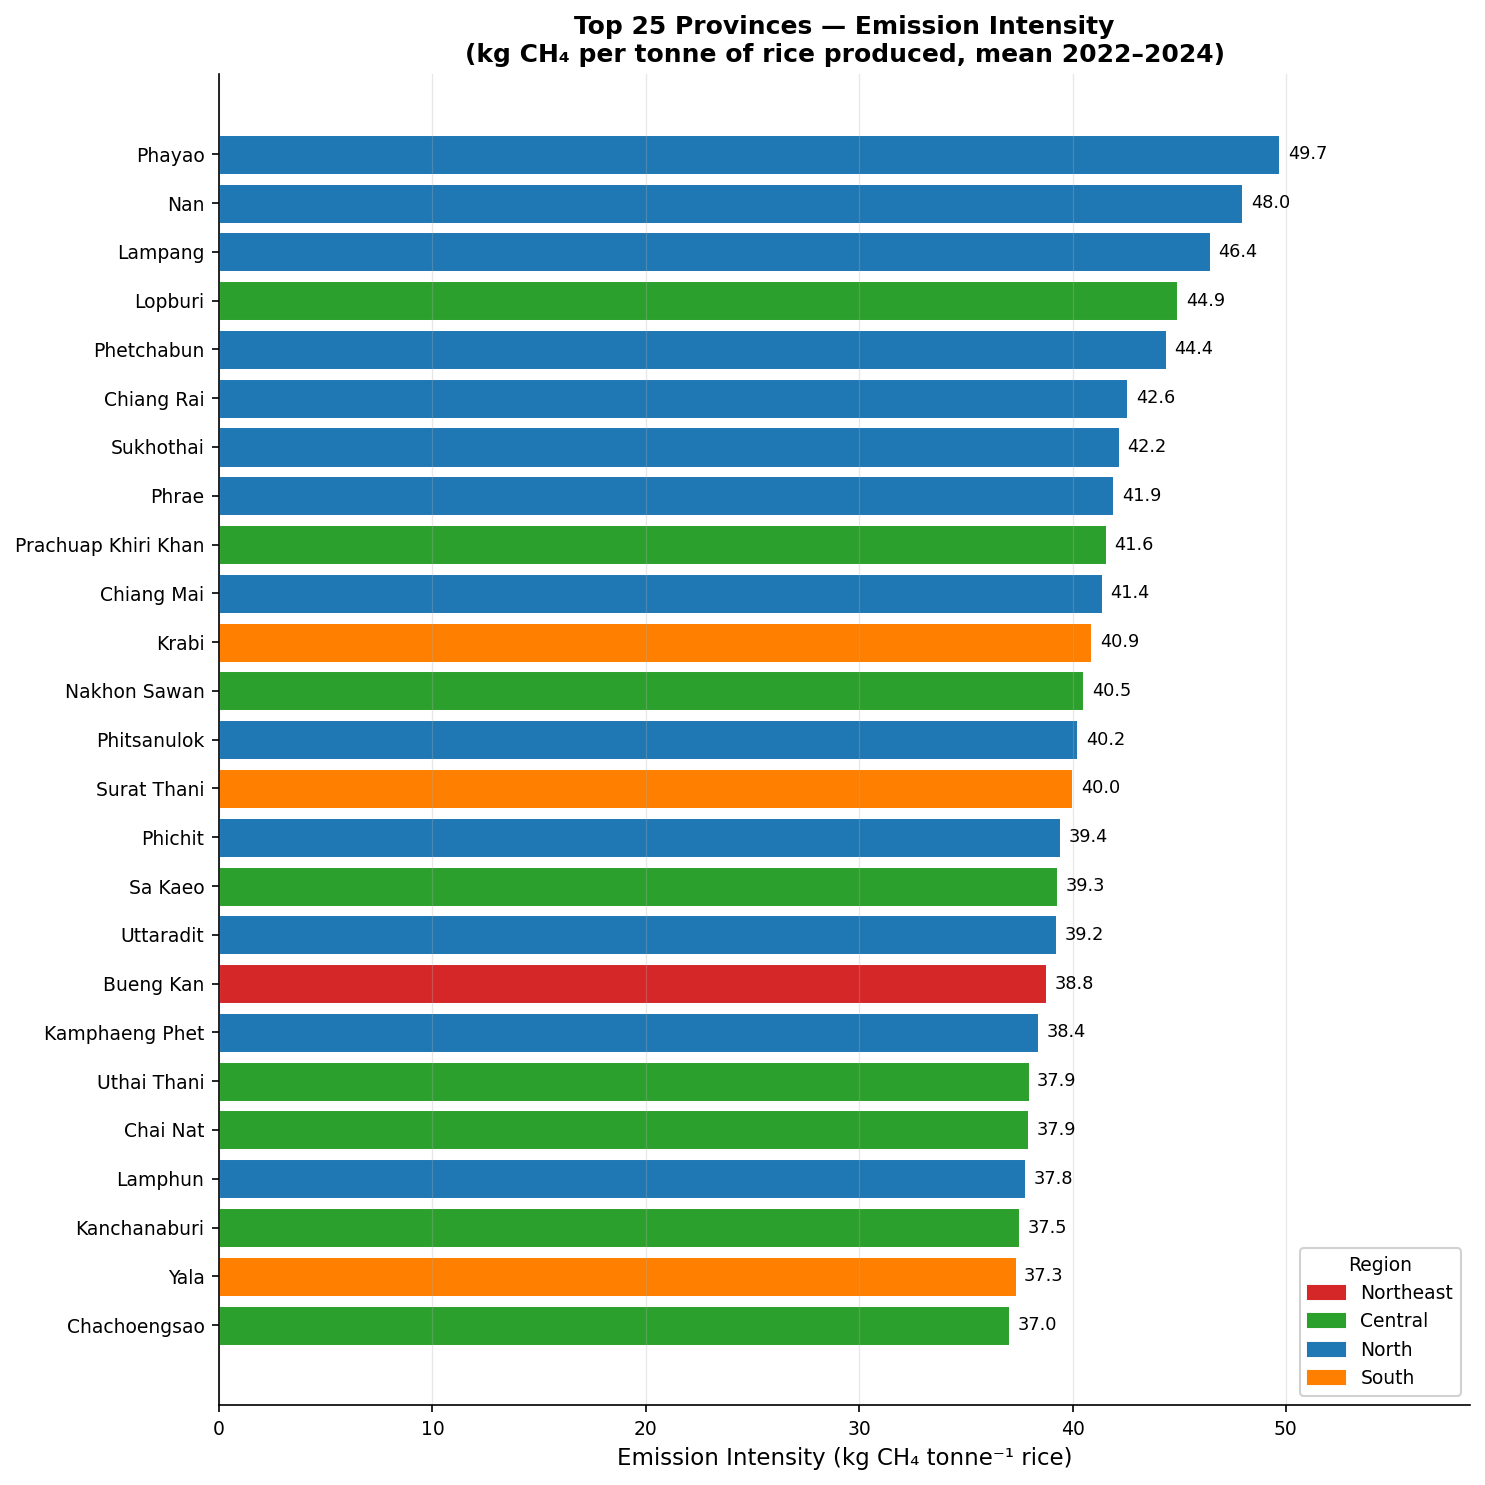
\includegraphics[width=0.78\linewidth]{plot5_intensity.png}
\caption{Top 25 provinces ranked by emission intensity
         (kg~CH\textsubscript{4}~t\textsuperscript{-1} rice produced),
         Thailand, mean 2022--2024.
         High intensity reflects low emission efficiency per unit food output.
         Source: \cite{oae2024}; authors' calculation.}
\label{fig:intensity}
\end{figure}

Figure~\ref{fig:intensity} reveals a striking reversal from the total-emission
picture.
The Northeast dominates national CH\textsubscript{4} \textit{by volume}
because it cultivates the most land, but it is \textbf{not} the most
carbon-inefficient region per tonne of rice produced.
That distinction belongs to \textbf{Southern provinces}---\textbf{Krabi}
(78.6~kg~t\textsuperscript{-1}), \textbf{Surat Thani} (76.9), and
\textbf{Phang Nga} (71.1)---and to the Eastern border province of
\textbf{Sa Kaeo} (75.5~kg~t\textsuperscript{-1}), all of which sit above
every Northeast province on the intensity ranking.

The explanation is the same mechanism in more extreme form: rice in these
provinces is a \textit{marginal} crop.
Southern farmers grow paddy in small, isolated plots amid rubber plantations
and oil palm, with no irrigation infrastructure and traditional low-yielding
varieties.
Sa Kaeo, despite its Central administrative classification, sits on the
Cambodian border beyond the reach of the Chao Phraya irrigation network and
behaves agronomically like a rainfed Northeast province.
In all these cases, the fields flood for a full season and emit CH\textsubscript{4}
at the same per-hectare rate as anywhere else, but they produce so little rice
per hectare that the methane cost per tonne is exceptionally high.
They are small emitters in absolute terms---their total areas are modest---but
they represent the most climate-inefficient rice production in the country.

The Northeast, by contrast, sits in the 63--69~kg~t\textsuperscript{-1}
band: high intensity relative to the irrigated Central Plains
(39--41~kg~t\textsuperscript{-1}), but not the worst.
The Khorat Plateau covers roughly 155{,}000~km\textsuperscript{2} of flat
terrain farmed as rainfed paddy for generations; large area at moderate yield
drives high \textit{total} emissions, not the highest per-tonne cost.
The Central and North irrigated provinces pay the lowest climate price per
tonne because reliable water, improved varieties, and double-cropping push
yields high enough to spread the fixed CH\textsubscript{4} cost across far
more rice.
In short: \textbf{volume and efficiency tell different stories about where
Thailand's rice emissions come from, and both stories matter for policy.}
These spatial patterns, however, are not fixed: price policy can drive
sharp year-to-year swings in cultivated area and thus total emissions.

\FloatBarrier
\subsection*{Econometrics: price policy as an emission driver}

Geography explains \textit{where} Thailand's rice emissions come from;
price policy explains \textit{when} they spike.
Figure~\ref{fig:policy} overlays farm-gate paddy price, yield, and estimated
CH\textsubscript{4} emissions from 2007 to 2024, annotated with key policy
events; the co-movement between price and CH\textsubscript{4} is immediate and striking.

\begin{figure}[!htbp]
\centering
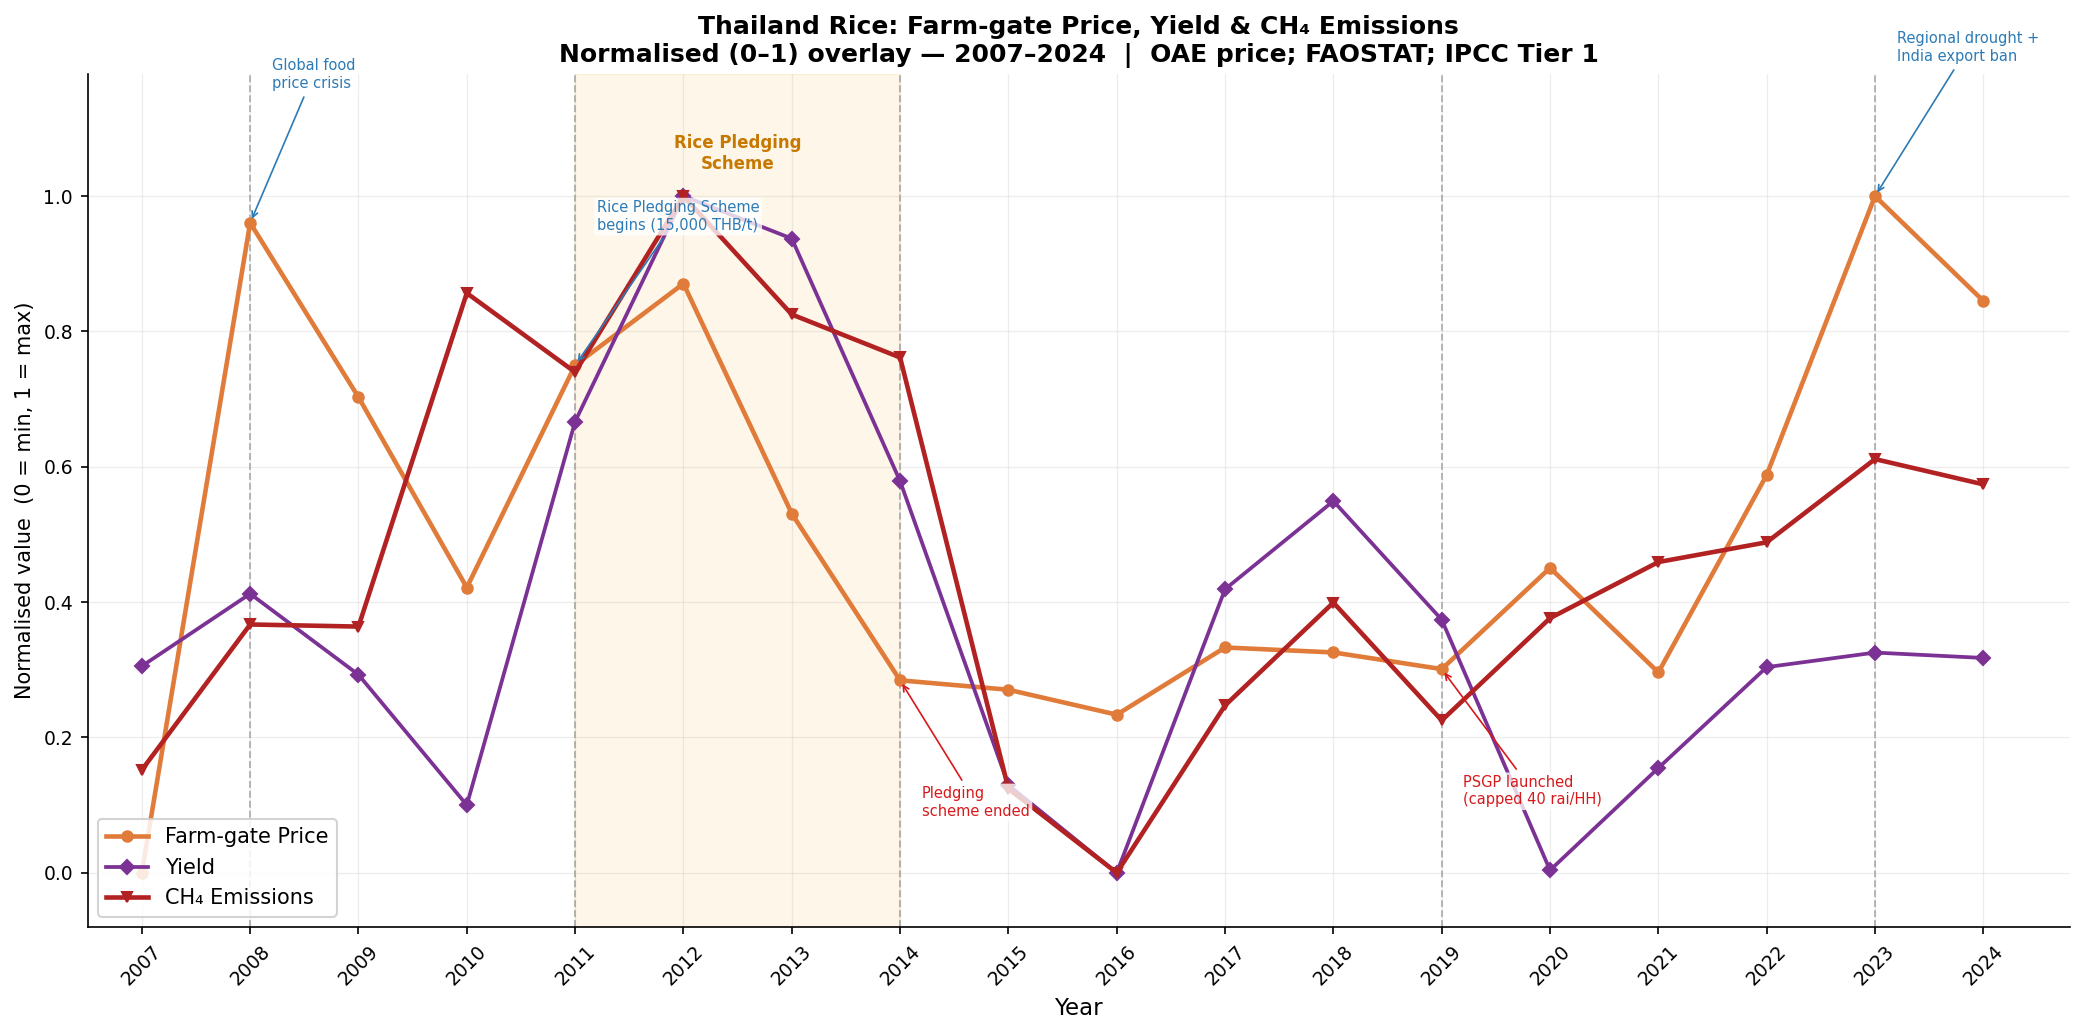
\includegraphics[width=0.96\linewidth]{plot6_policy_timeline.png}
\caption{Thailand rice farm-gate price (THB~tonne\textsuperscript{-1}),
         yield (hg~ha\textsuperscript{-1}), and estimated CH\textsubscript{4}
         emissions (Gg~yr\textsuperscript{-1}), normalised (0--1), 2007--2024.
         Vertical dashed lines mark major policy events.
         Sources: \cite{oae2024} (price); \cite{faostat2026}; authors' calculation.}
\label{fig:policy}
\end{figure}

The price time series shows three distinct periods.
During \textbf{2008}, the global food price crisis briefly doubled farm-gate
prices (6,600 to 10,500~THB~tonne\textsuperscript{-1}), triggering a modest
area expansion.
The most pronounced episode is the \textbf{Rice Pledging Scheme}
(\textit{khrongkan rap chamnam khao}; 2011--2014), introduced as an electoral
commitment by the Pheu Thai government.
The scheme obliged the government to purchase \textit{all} paddy offered by
farmers at 15,000~THB~tonne\textsuperscript{-1} for white rice and
20,000~THB~tonne\textsuperscript{-1} for jasmine, approximately 40--50\%
above world market prices, with \textbf{no quantity cap per
household} \citep{poapongsakorn2014}.
This design created an unlimited expansion incentive: every additional tonne
planted was guaranteed to be profitable regardless of market conditions.
Farmers responded rationally by converting non-rice land to paddy, expanding
double-cropping in irrigated areas, and pushing marginal fields into production.
National harvested area reached record levels and CH\textsubscript{4} reached
its 64-year peak of \textbf{1,884~Gg in 2012}.

The scheme ultimately became fiscally unsustainable.
The government purchased approximately 52\% of total national paddy production
but could not resell stockpiles on world markets: Thai offer prices were too
high relative to competing exporters \citep{usda2017}.
Warehoused rice deteriorated, widespread corruption in storage contracts
emerged, and the total programme cost reached \textbf{984~billion~THB}
(approximately USD~32~billion), equivalent to 41\% of the 2013 national
budget \citep{poapongsakorn2014, usda2017}.
Following the May 2014 military coup, the incoming government cancelled the
scheme; farm-gate prices fell sharply and harvested area contracted by over
5\% in 2014/15, pulling CH\textsubscript{4} downward proportionally.
This sequence---policy introduced, emissions spike, policy cancelled, emissions
fall---is consistent with a causal interpretation, though formal proof would
require a counterfactual comparison region or a more complete model.

Since 2015, the government has operated a lighter-touch \textbf{Price Subsidy
Guarantee Programme} (PSGP), which pays farmers the difference between a
reference price and the market price, capped at 40~rai (6.4~ha) per household.
This redesign shows a key principle: \textit{how} a price-support programme
is structured matters as much as the price level itself.
The Pledging Scheme's unlimited guarantee made every extra hectare profitable
no matter what, a direct incentive to expand.
The PSGP's per-household cap removes that incentive beyond 6.4~ha, limiting
the land-expansion response.
Since 2019, price and area trajectories have been more stable, showing that
climate-friendly policy design does not require abandoning farmer income support.

\FloatBarrier
\subsection*{The counterfactual: emission costs of uncapped guarantees}

\textbf{Counterfactual: the emission cost of programme design.}
The regression dummy coefficient ($\hat{\beta}_2 = 988$~kha) isolates the
structural expansion effect of the unlimited guarantee, the excess area beyond
what the contemporaneous farm-gate price alone would predict.
This provides a direct basis for a counterfactual: \textit{had the Pledging
Scheme included the same 40-rai (6.4~ha) per-household cap as the current PSGP,
this structural expansion would have been constrained.}
Applying the main-season emission factor, the estimated \textbf{avoided
CH\textsubscript{4} is 151.6~Gg~yr\textsuperscript{-1}}, equivalent to 10.7\%
of the long-run national mean, for each year the cap would have been in effect.
Summed across the scheme's four-year duration (2011--2014), the cap would have
prevented approximately \textbf{606~Gg~CH\textsubscript{4}} (17.0~Mt~CO\textsubscript{2}e).
For context, this exceeds the maximum annual AWD mitigation potential estimated
in this study (124.1~Gg at a 50\% EF reduction) by a factor of nearly five per
scheme year, meaning one structural design choice in 2011 generated more
cumulative emission impact than a decade of nationwide AWD adoption would save.
This comparison does not argue against AWD; rather, it illustrates the
\textit{relative} leverage of programme-design decisions versus field-level
mitigation technologies.
The counterfactual should be read as an upper-bound estimate for two reasons.
First, the cap would bind only for households already operating above 6.4~ha;
smallholders below that threshold would be unaffected and their price-driven
expansion would continue.
Second, capped subsidy schemes in Thailand have documented instances of
land-title subdivision, where households divide holdings among family members
to remain under the cap threshold, a behavioural response that would partially
erode the cap's effectiveness in practice \citep{poapongsakorn2014}.
The 2023 spike in price (10,700~THB~tonne\textsuperscript{-1}) reflects
regional drought reducing supply combined with elevated
global export demand following the India rice export ban.

Statistical analysis confirms a \textbf{significant positive relationship}
between farm-gate price and harvested area ($r = 0.505$, $p = 0.033$, $n = 18$).
A regression slope of 0.045~Gg~CH\textsubscript{4} per THB~tonne\textsuperscript{-1}
(derived from the area--price slope of 291~ha per THB~tonne\textsuperscript{-1})
implies that a 1,000~THB~tonne\textsuperscript{-1} sustained price increase
is associated with approximately 45~Gg additional CH\textsubscript{4}~yr\textsuperscript{-1},
equivalent to about 2.6\% of the 2024 national total.

\begin{table}[!htbp]
\centering
\caption{Regression of national harvested area on price and Pledging Scheme
         dummy, Thailand, 2007--2024 ($n = 18$). Dependent variable: national
         harvested area (ha). $D_t = 1$ for 2011--2014, 0 otherwise.
         HAC standard errors use Newey--West estimator (maxlags = 1)
         \citep{neweywest1987}.}
\label{tab:dummy}
\begin{tabular}{@{}lrrr@{}}
\toprule
 & \textbf{Model 1} & \textbf{Model 2} & \textbf{Model 2 (HAC)} \\
 & \textit{Price only} & \textit{Price + dummy} & \textit{NW SE} \\
\midrule
Intercept      & 8{,}490{,}000 ha & 8{,}869{,}000 ha & 8{,}869{,}000 ha \\
Price ($\hat{\beta}_1$, ha/THB~t\textsuperscript{-1}) & 291 & 222 & 222 \\
\quad $p$-value            & 0.033 & 0.029 & \textbf{0.005} \\
Pledging dummy ($\hat{\beta}_2$, kha) & --- & $+$988 & $+$988 \\
\quad $p$-value            & --- & 0.001 & \textbf{$<$0.001} \\
\midrule
$R^2$                       & 0.255 & 0.631 & --- \\
$\Delta R^2$                & ---   & $+$0.376 & --- \\
Durbin--Watson              & 1.162 & 2.141 & --- \\
\bottomrule
\multicolumn{4}{@{}l@{}}{\footnotesize CH\textsubscript{4} equivalent of $\hat{\beta}_2$: 151.6~Gg~yr\textsuperscript{-1} (EF = 153.4~kg~ha\textsuperscript{-1}, \citealt{buddhaboon2011}).} \\
\multicolumn{4}{@{}l@{}}{\footnotesize DW $\approx$ 2 for Model~2 indicates autocorrelation resolved once dummy is included.}
\end{tabular}
\end{table}

To test whether the Pledging Scheme expanded area beyond the price effect
alone, a policy dummy ($D_t = 1$ for 2011--2014) was added to the regression
(Equation~\ref{eq:dummy}; Table~\ref{tab:dummy}).
Adding the dummy raises $R^2$ from 0.255 to 0.631.
The dummy coefficient ($\hat{\beta}_2 = 988$~kha) shows that the Pledging
Scheme years are linked to roughly \textbf{988,000 additional hectares}
beyond what price alone explains, equivalent to
\textbf{151.6~Gg~CH\textsubscript{4}~yr\textsuperscript{-1}}
(4,245~Gg~CO\textsubscript{2}e).
The price slope also drops from 291 to 222~ha per THB~tonne\textsuperscript{-1}
once the dummy is included, showing the simpler model was blending the
scheme's direct area effect with the general price response.
Both effects remain highly significant under Newey--West HAC standard errors
\citep{neweywest1987} ($p_{\text{price}} = 0.005$;
$p_{\text{pledging}} < 0.001$).
The dummy coefficient should be read as capturing the scheme's \textit{combined}
effect (both the price premium and the structural guarantee of unlimited
government purchasing) rather than a clean separation of the two, given that
$D_t$ and $P_t$ are correlated during the 2011--2014 pledge years.

\FloatBarrier
\subsection*{Forward-looking mitigation: targeting AWD in irrigated systems}

\begin{figure}[!htbp]
\centering
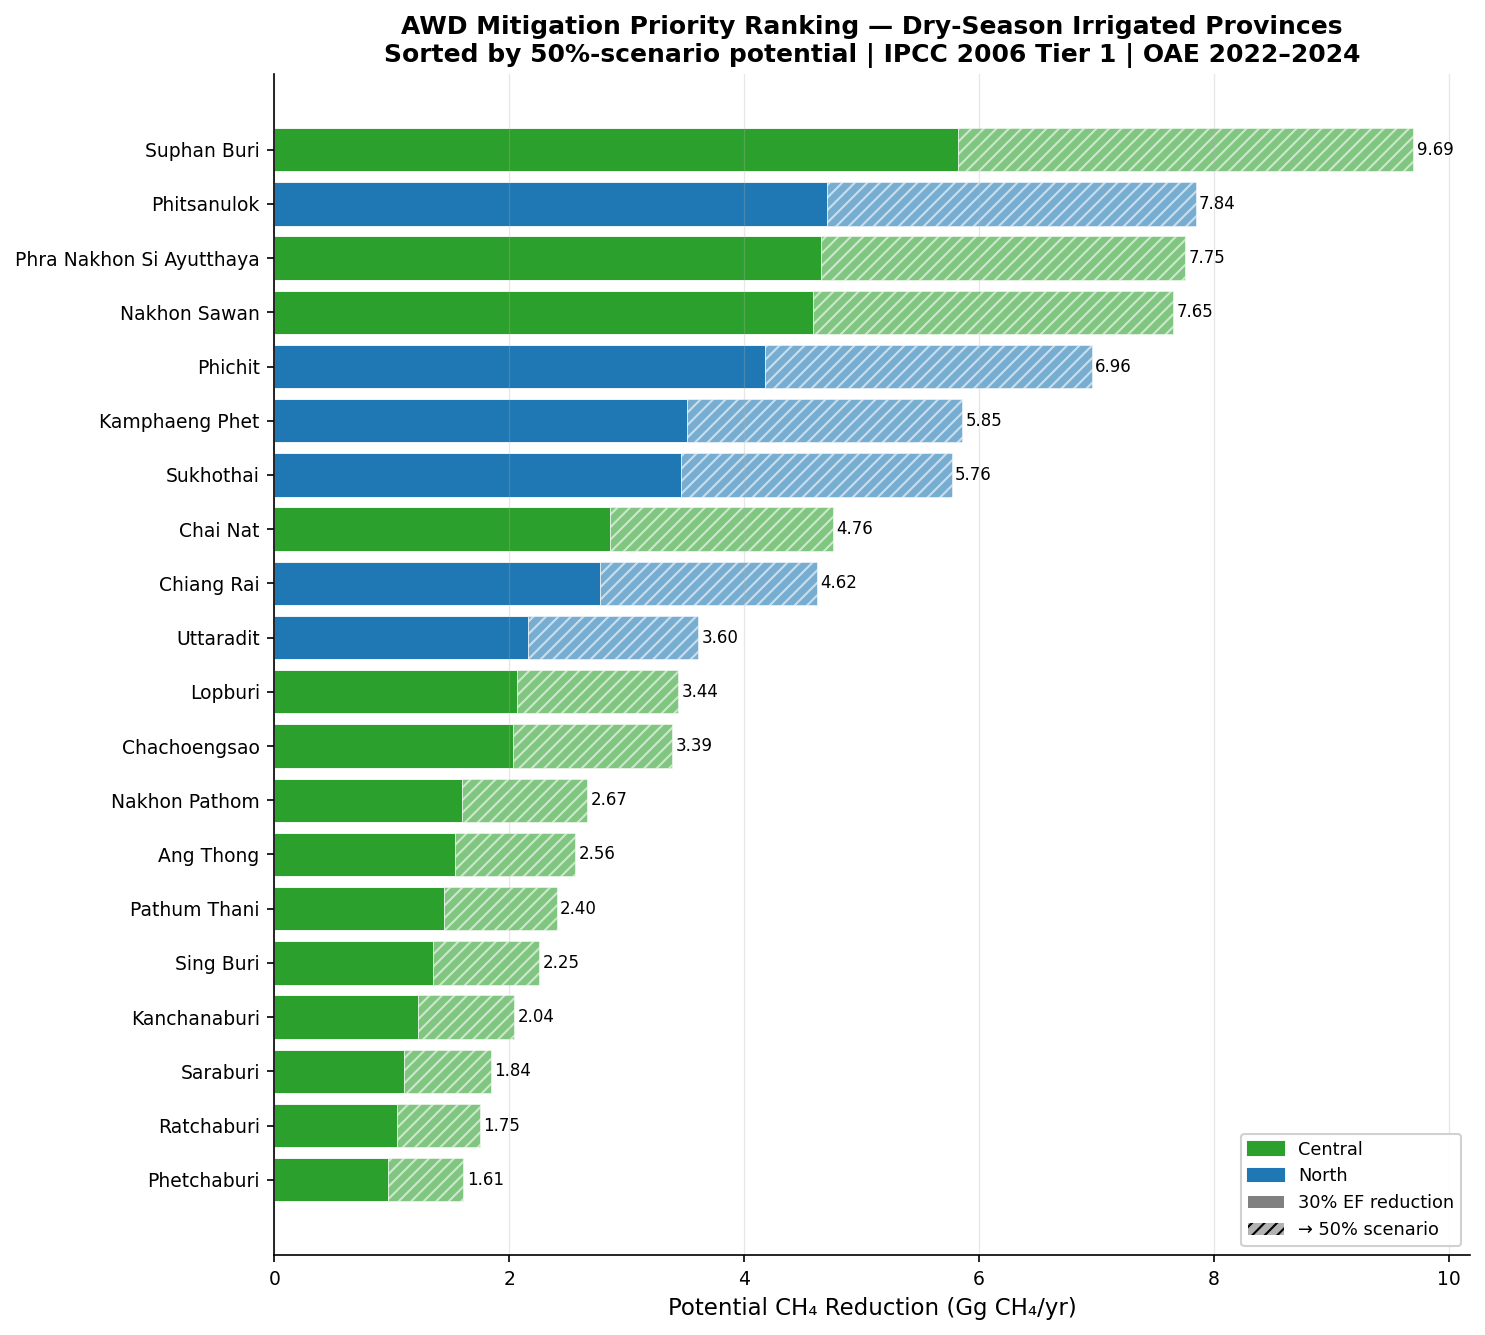
\includegraphics[width=0.96\linewidth]{plot9_awd_priority.png}
\caption{AWD mitigation priority ranking by province.
         Bars show potential CH\textsubscript{4} reduction under 30\% (solid)
         and 50\% (hatched extension) EF reduction scenarios applied to
         dry-season irrigated area only.
         Bar colour indicates macro-region.
         Source: \cite{oae2024}; \cite{sander2014}; authors' calculation.}
\label{fig:awd}
\end{figure}

These findings have direct policy implications.
First, \textbf{price-support programmes must account for their emission
co-effects}: purchasing guarantees that raise farm-gate prices above equilibrium
will expand the cultivated area and increase CH\textsubscript{4} proportionally.
Emission impact assessments should be a standard component of rice subsidy
design under Thailand's NDC framework.
Second, \textbf{targeted adoption of Alternate Wetting and Drying (AWD)},
which involves intermittent drainage during the growing season, could cut per-hectare CH\textsubscript{4}
by 30--50\% without yield loss \citep{sander2014, wassmann2000}.
AWD is applicable only to the dry-season irrigated area, where water control
infrastructure enables scheduled drainage.
Province-level analysis of dry-season harvested area (Figure~\ref{fig:awd})
identifies \textbf{Suphan Buri}, \textbf{Phitsanulok}, \textbf{Phra Nakhon Si Ayutthaya},
and \textbf{Nakhon Sawan} as the highest-priority provinces, together accounting
for 32\% of national AWD mitigation potential.
Applying a conservative 30\% EF reduction to all provinces with dry-season
irrigated paddy yields a national reduction of \textbf{74.6~Gg~yr\textsuperscript{-1}}
(4.3\% of the 2024 total); a 50\% reduction saves \textbf{124.1~Gg~yr\textsuperscript{-1}}
(7.2\%).
These estimates supersede the coarser Central Plains regional aggregates used
in earlier versions and reflect the actual dry-season irrigated footprint across
all 77 provinces.
Extending AWD incentives through carbon credit mechanisms tied to Thailand's NDC
represents a priority opportunity \citep{thailand_ndc2022}.
Critically, Thailand's evolving price-support architecture offers a direct
implementation lever: embedding AWD compliance as a prerequisite for PSGP subsidy
payments would align income transfers with climate outcomes, delivering
CH\textsubscript{4} reductions precisely in the irrigated areas where water
control is feasible and programme monitoring is most practicable.

Three concrete policy steps follow from this analysis.
First, AWD adoption should be \textbf{prioritised} in Suphan Buri, Phitsanulok,
Phra Nakhon Si Ayutthaya, and Nakhon Sawan, the four provinces that together
account for the largest share of national AWD mitigation potential and already
operate the irrigation infrastructure required for scheduled drainage.
Second, AWD compliance should be made a \textbf{mandatory condition} for
PSGP subsidy receipt rather than a voluntary option, using OAE's existing
plot-level monitoring to verify adoption without creating a parallel
bureaucracy.
Third, verified AWD emission reductions should be linked to Thailand's
\textbf{domestic carbon market} or international climate finance instruments
under the NDC framework \citep{thailand_ndc2022}, giving irrigated-area
farmers a direct monetary incentive that complements the income guarantee.
Together, these steps would use the same PSGP administrative architecture
that already caps area expansion to additionally mandate cleaner water
management, turning a single programme into a dual lever for income support
and climate compliance.
Third, given that the Northeast simultaneously has the largest total emissions
and the highest emission intensity per tonne, \textbf{policy instruments that raise Northeast yields}
(improved drought-tolerant varieties, supplemental irrigation)
would reduce intensity even without changing area.

\subsection*{Limitations and uncertainties}

The biggest source of uncertainty in this study is probably the water management
assumption.
Tier~1 sets $\text{SF}_w = 1.0$ for all fields, which treats a continuously
flooded Central Plains paddy the same as a rainfed Northeast field that dries
out between monsoon events.
In practice, IPCC Table~5.12 puts $\text{SF}_w$ as low as 0.28 for
intermittently rainfed conditions, meaning the Northeast figures here could be
overestimates by a factor of three or four, while Central Plains emissions may
be underestimated.
I was unable to obtain province-level water management data to apply Tier~2
scaling factors, so Northeast emission numbers should be read as upper-bound
estimates rather than central values.
Applying the IPCC Table~5.12 default $\text{SF}_w = 0.28$ for intermittently
rainfed conditions to the Northeast's 6,060~kha would reduce its estimated
contribution from 927.0~Gg to approximately 259~Gg, cutting the national
total by roughly 39\%.
This study's national baseline of 1,420~Gg~yr\textsuperscript{-1} is therefore
best interpreted as a Tier~1 upper bound pending field-based water management
surveys.

The uniform cultivation period (118 days main season, 111 days dry season,
\citealt{buddhaboon2011}) is a second simplification.
Real season lengths vary by province and variety (roughly $\pm$10 days in
either direction), and province-level data to differentiate them remain limited.
Table~\ref{tab:sensitivity} shows how national emissions shift across a
plausible $\pm$20\% range in $\text{EF}_c$ combined with $\pm$10 days in
season length, giving a mean range of 1,040--1,848~Gg~yr\textsuperscript{-1}
and a 2024 range of 1,263--2,247~Gg~yr\textsuperscript{-1}.

\begin{table}[!htbp]
\centering
\caption{Sensitivity of national $\mathrm{CH}_{4}$ estimates to $\mathrm{EF}_{c}$ and season length ($t_{p}$) assumptions.}
\label{tab:sensitivity}
\begin{tabular}{@{}lrrrrrr@{}}
\toprule
\textbf{Scenario} &
  \textbf{EF\textsubscript{c}} &
  \textbf{$t_p$} &
  \textbf{EF} &
  \textbf{Mean} &
  \textbf{2024} &
  \textbf{Change} \\
 &
  (kg~ha\textsuperscript{-1}~d\textsuperscript{-1}) &
  (days) &
  (kg~ha\textsuperscript{-1}) &
  (Gg~yr\textsuperscript{-1}) &
  (Gg~yr\textsuperscript{-1}) &
  (\%) \\
\midrule
Low  ($-$20\% $\text{EF}_c$, $-$10 d) & 1.04 & 108 & 112.3 & 1,040.0 & 1,263.0 & $-$27 \\
\textbf{Central (baseline)}            & \textbf{1.30} & \textbf{118} & \textbf{153.4} & \textbf{1,420.0} & \textbf{1,725.5} & --- \\
High ($+$20\% $\text{EF}_c$, $+$10 d) & 1.56 & 128 & 199.7 & 1,848.5 & 2,246.8 & $+$30 \\
\bottomrule
\multicolumn{7}{@{}l@{}}{\footnotesize EF = $\text{EF}_c \times t_p$; applied to FAOSTAT harvested area.}
\end{tabular}
\end{table}
The price--area regression is the part I am least confident about.
Eighteen years of data is not much, and drought years such as 2015--16 are
a good example of why: area fell sharply despite prices holding steady,
a drop the model attributes partly to price when the real driver was
rainfall failure.
Export demand and input costs are also correlated with farm-gate price but
are not separately controlled for, so the price coefficient likely captures
some of that confounding.
A longer time series with explicit climate and trade controls would help
disentangle these effects; for now the regression is best read as a
reduced-form association rather than a clean structural estimate.
Field-measured, province-specific emission factors would address the Tier~1
uncertainties on the methods side \citep{wassmann2000, yan2009}.
A natural extension of this work is a dedicated Tier~2 study applying
province-level $\text{SF}_w$ values from field campaigns across Thailand's
major water-management regimes.
Under Tier~2, the Northeast's emissions would likely fall substantially
(SF\textsubscript{w} = 0.28 for intermittently rainfed conditions implies a
roughly three- to four-fold reduction relative to the Tier~1 estimate),
while the Central Plains, with its fully irrigated, continuously flooded
paddies, would emerge as the dominant emitting region.
Such a spatial reordering would validate the AWD priority ranking derived
here (which already targets Central Plains provinces) while substantially
revising the absolute magnitudes and the relative importance of Northeast
yield-improvement recommendations.
Finally, while the policy section proposes embedding AWD compliance as a
condition for PSGP subsidy receipt, implementing this credibly requires
monitoring infrastructure beyond what currently exists: scheduled drainage
must be documented through water-level sensors, soil moisture records, or
sufficiently high-resolution remote sensing, none of which OAE's current
plot-area surveys provide.
MRV build-out costs should therefore be evaluated against mitigation benefits
before mandatory conditionality is adopted.

% =============================================================
\section*{Conclusions}
% =============================================================

Thai rice paddies are a significant and growing source of agricultural
methane, but one whose trajectory is shaped more by the structural design
of price-support programmes than by either agronomic improvement or
field-level mitigation technology.
The central finding of this study is that a single design choice (the absence
of a per-household area cap in the 2011--2014 Rice Pledging Scheme) is
estimated to have generated 606~Gg~CH\textsubscript{4} (17.0~Mt~CO\textsubscript{2}e)
of avoidable emissions over four years, exceeding the annual mitigation
potential of full AWD adoption across all irrigated provinces by a factor of five.
The practical implication is that Thailand's path to meeting its NDC
agriculture targets runs primarily through the design of its next rice
price-support programme, not through yield improvement or AWD alone.
The key findings of this study are:

\begin{enumerate}[noitemsep]
  \item National emissions increased significantly at +12.0~Gg~yr\textsuperscript{-1}
        ($R^2 = 0.830$, $p < 0.001$) over 1961--2024, peaking at 1,884~Gg in 2012
        and reaching 1,726~Gg (48.3~Mt~CO\textsubscript{2}e) in 2024.

  \item The Northeast dominates provincial emissions (54.9\%, 927.0~Gg~yr\textsuperscript{-1}),
        driven by its large harvested area; \textbf{Ubon Ratchathani} is the
        highest-emitting province (101.4~Gg~yr\textsuperscript{-1}).

  \item National emission intensity declined from 92.5 to 51.4~kg~CH\textsubscript{4}~t\textsuperscript{-1}
        ($-$44\%; $R^2 = 0.892$, $p < 0.001$), reflecting a genuine food-system efficiency gain
        as yield growth outpaced area expansion.
        This is \textit{relative} decoupling only: absolute emissions rose 84\% over the
        same period, and per-hectare flux is unchanged under Tier~1's constant EF.

  \item Emission intensity is highest in Northeast provinces
        (63--69~kg~CH\textsubscript{4}~t\textsuperscript{-1} under Tier~1 assumptions),
        reflecting the yield penalty of rainfed cultivation.
        These figures are upper bounds: IPCC Table~5.12 $\text{SF}_w$ values
        of 0.28 for rainfed conditions would substantially reduce
        Northeast emissions under a Tier~2 framework.
        Subject to that refinement, Northeast provinces are candidate targets
        for yield improvement programmes that would reduce emission intensity.

  \item Farm-gate price is a significant positive predictor of harvested area
        ($r = 0.505$, $p = 0.033$, $n = 18$); the 2011--2014 Rice Pledging Scheme
        added $\sim$988,000~ha beyond the price effect alone, consistent with a
        policy-induced area expansion driving the 2012 emission peak.

  \item \textbf{Programme design determines emission risk more than price level.}
        A counterfactual cap-equivalent calculation estimates that a 40-rai
        per-household limit applied from 2011 would have avoided
        \textbf{606~Gg~CH\textsubscript{4}} (17.0~Mt~CO\textsubscript{2}e)
        over the scheme's four-year duration, exceeding five times the annual
        AWD mitigation potential.
        Future price-support programmes should treat area cap design as a
        primary climate-policy variable, not an afterthought.

  \item \textbf{Yield improvement does not automatically reduce absolute emissions.}
        Emission intensity fell 44\% over 1961--2024 as yields improved, yet
        absolute emissions rose 84\% because yield gains raised the profitability
        of rice farming and attracted area expansion (rebound effect).
        The 2012 emission peak coinciding with Thailand's lowest-ever emission
        intensity (47.7~kg~t\textsuperscript{-1}) illustrates this directly.
        Absolute CH\textsubscript{4} reduction requires either area contraction
        or water management change; yield improvement alone is insufficient and
        may be counterproductive when paired with uncapped price guarantees.

  \item AWD adoption across dry-season irrigated provinces reduces national
        CH\textsubscript{4} by 5--8\% under 30--50\% EF reduction scenarios,
        with Central Plains provinces (led by Suphan Buri and Phitsanulok)
        accounting for the largest share of mitigation potential.
        Embedding AWD compliance as a condition for PSGP subsidy receipt
        represents the most actionable mitigation pathway under Thailand's NDC.
\end{enumerate}

% =============================================================
\section*{Acknowledgements}

The authors thank the Food and Agriculture Organization of the United Nations
for FAOSTAT data access, and the Office of Agricultural Economics, Ministry of
Agriculture and Cooperatives, Thailand, for provincial rice statistics and
price data.

% =============================================================
\section*{AI Use Disclosure}

Claude (Anthropic), an AI language model, was used during the preparation of
this manuscript to assist with prose editing, structural feedback, and LaTeX
formatting.
All data collection, emission calculations, statistical analysis, and
intellectual conclusions are the author's own.
The author takes full responsibility for the accuracy and integrity of the
content presented.

% =============================================================
\section*{Appendix}
% =============================================================

\begin{figure}[!htbp]
\centering
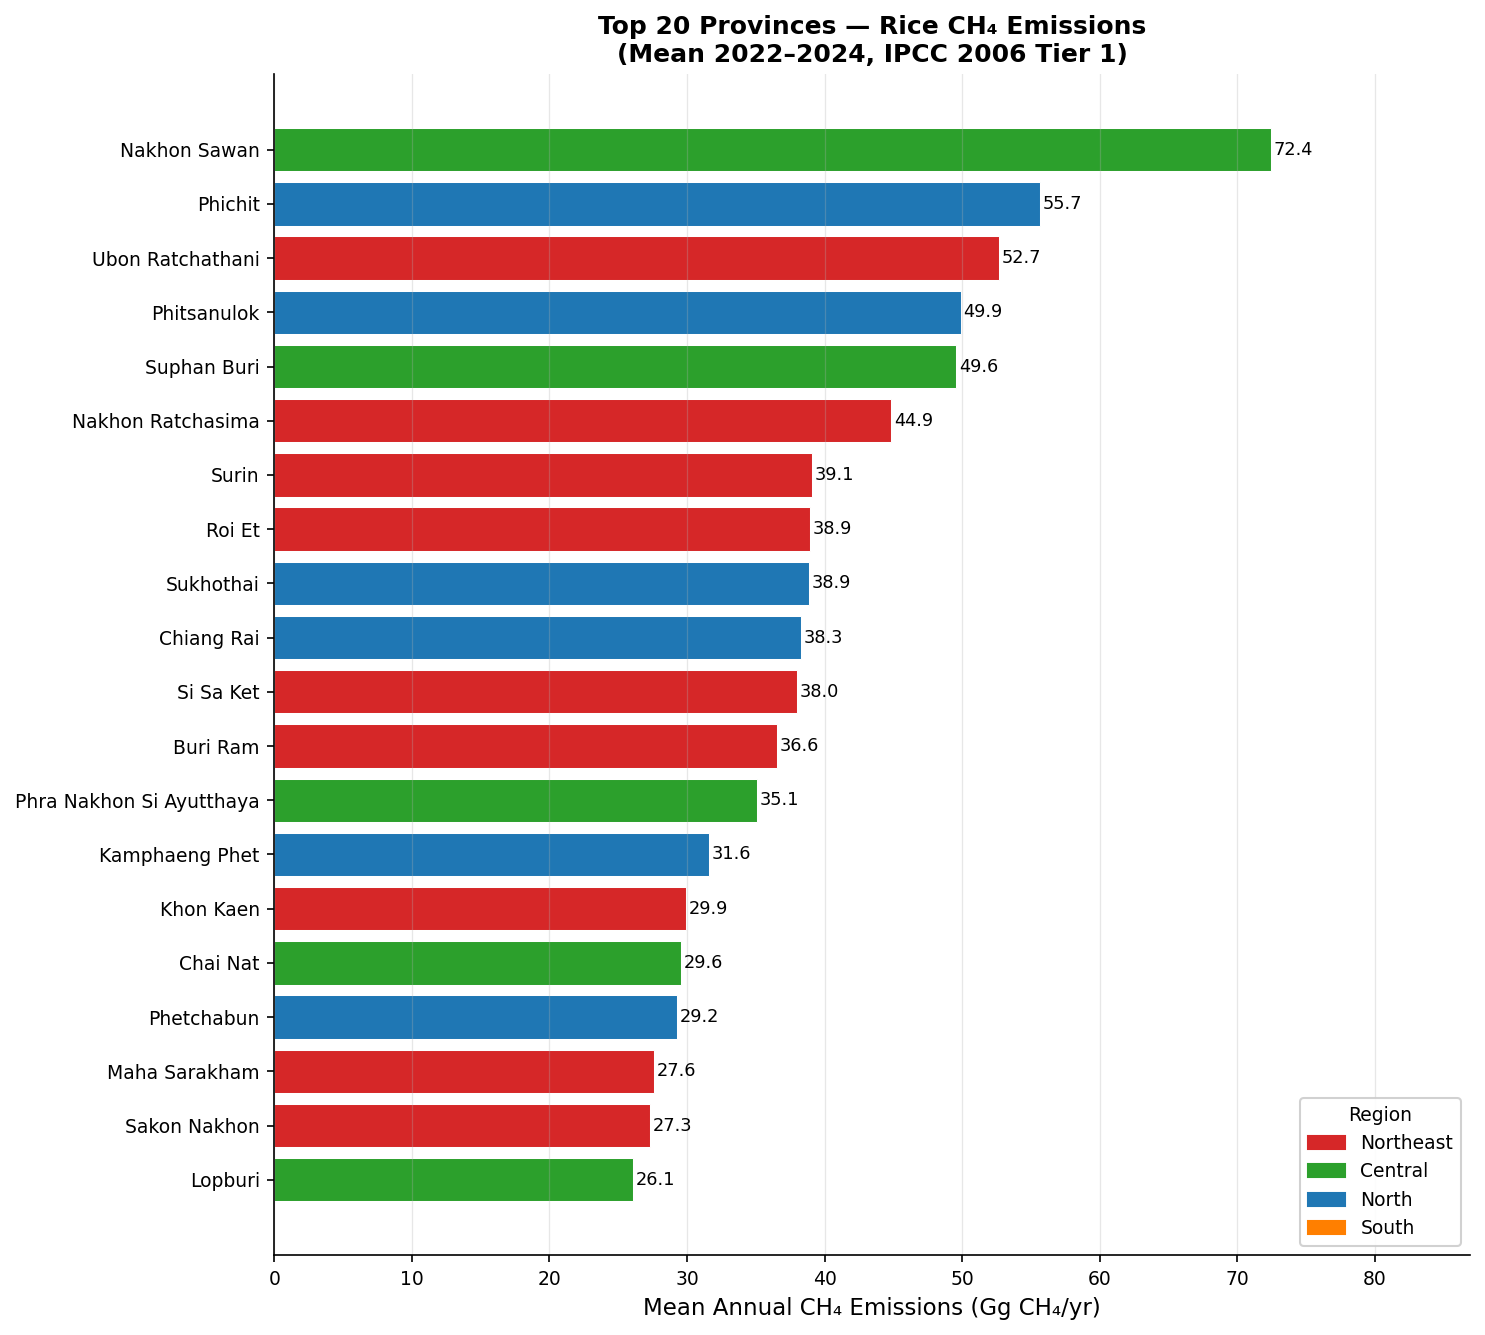
\includegraphics[width=0.96\linewidth]{plot2_top20_provinces.png}
\caption{Top 20 provinces ranked by mean annual rice CH\textsubscript{4}
         emissions, 2022--2024. Bar colour indicates macro-region.
         Source: \cite{oae2024}; authors' calculation.}
\label{fig:top20}
\end{figure}

\begin{figure}[!htbp]
\centering
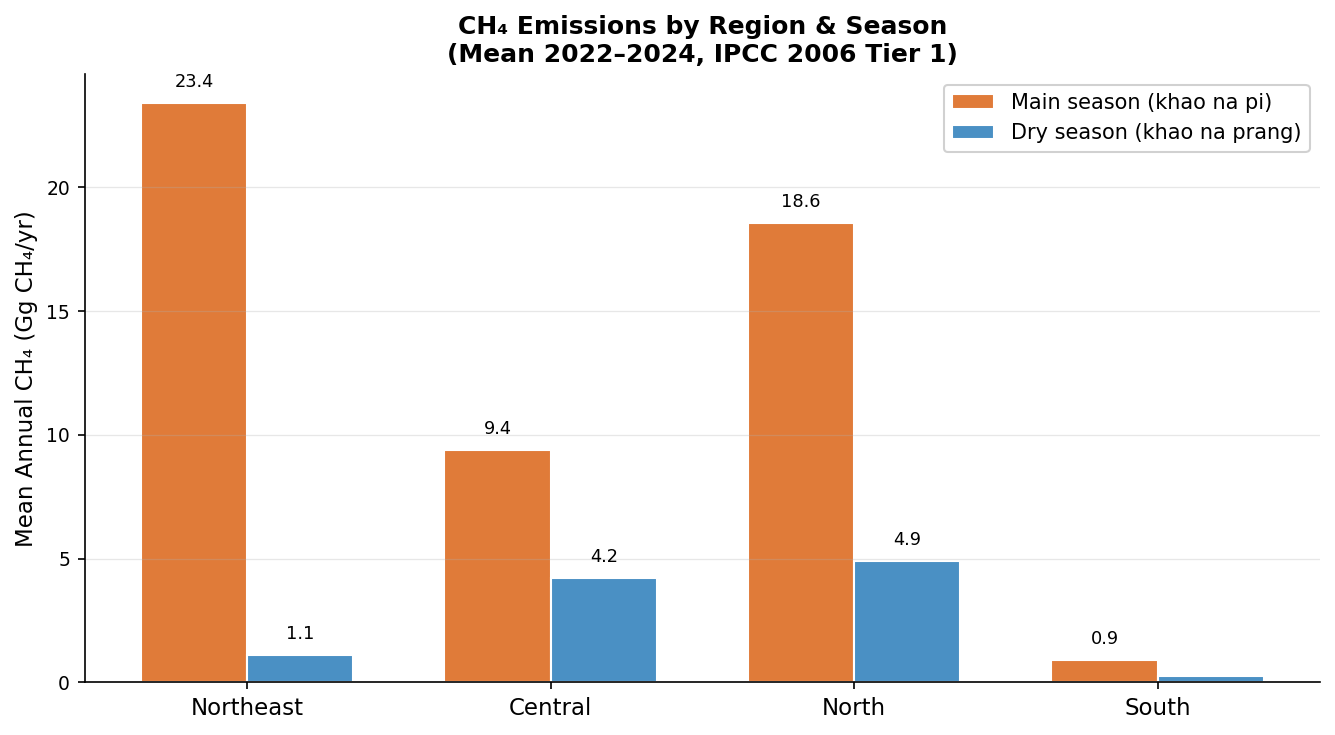
\includegraphics[width=0.92\linewidth]{plot3_region_season.png}
\caption{Mean annual rice CH\textsubscript{4} emissions \textbf{per province}
         by region and season, Thailand, 2022--2024.
         Orange: main season (\textit{khao na pi});
         blue: dry season (\textit{khao na prang}).
         Source: \cite{oae2024}; authors' calculation.}
\label{fig:region}
\end{figure}

\begin{table}[!htbp]
\centering
\caption{Regional rice CH\textsubscript{4} emission summary,
         mean annual 2022--2024 (IPCC 2006 Tier~1).}
\label{tab:region}
\begin{tabular}{@{}lrrr@{}}
\toprule
\textbf{Region} &
  \textbf{Area (kha)} &
  \textbf{CH\textsubscript{4} (Gg)} &
  \textbf{Share (\%)} \\
\midrule
Northeast &  6,060 & 927.0 & 54.9 \\
Central   &  2,648 & 398.7 & 23.6 \\
North     &  2,225 & 336.8 & 19.9 \\
South     &    178 &  27.0 &  1.6 \\
\midrule
\textbf{Total} & \textbf{11,110} & \textbf{1,689.6} & \textbf{100.0} \\
\bottomrule
\end{tabular}
\end{table}

% =============================================================
\bibliography{references}

\end{document}
